\documentclass[a4paper,12pt]{article}
\usepackage[utf8]{inputenc}
\usepackage[Bigl=3cm,Bigl=3cm,top=3cm,bottom=3cm]{geometry}
\usepackage[T1]{fontenc}
\usepackage[french]{babel}
\usepackage{listings}
\usepackage{longtable}
\usepackage{graphicx}
\usepackage{fancyhdr}
\usepackage{multicol}
\usepackage{caption}
\usepackage{float}
\usepackage{tabularx}
\usepackage{fancybox}
\usepackage{eurosym}
\usepackage{hyperref}
\usepackage{wasysym}
\usepackage{titlesec}
\usepackage{xcolor}
\usepackage{listings}
\usepackage{enumitem}
\usepackage{listings}
\usepackage{color}
\usepackage{amsmath}
\usepackage{comment}
\usepackage{amssymb}
\definecolor{dkgreen}{rgb}{0,0.6,0}
\definecolor{gray}{rgb}{0.5,0.5,0.5}
\definecolor{mauve}{rgb}{0.58,0,0.82}

\pagestyle{fancy}
%\fancyhf{}
\rfoot{\textit{Projet}}
\lfoot{\textit{M2 ISF App}}
%\rfoot{}
\fancyfoot[C]{\thepage}
\titleformat{\section}[block]{\normalfont\Large\bfseries}{}{0pt}{}

% Configuration de l'en-tête
\fancypagestyle{plain}{
    \fancyhead[L]{\nouppercase{\rightmark}} % En-tête gauche avec le titre de la section sans numérotation
    \fancyhead[R]{
\includegraphics[width=30mm]{Dauphine.jpg}} % En-tête droite avec l'image
    \renewcommand{\headrulewidth}{0.4pt}
    \renewcommand{\footrulewidth}{0pt}
}

\pagestyle{plain}
\renewcommand{\sectionmark}[1]{\markright{#1}}
\begin{document}
\titleformat{\section}[block]{\normalfont\Large\bfseries}{}{0pt}{}

\begin{titlepage}

	\centering
	

    
    {Hayder Bouaziz - Eliott Brézet - Jianhyan Dong}
    \hfill
	{\large Année 2024/2025 \par}

	
	{\phantom o\par}
	\vspace{3cm}
	{\Huge\bfseries Python et Pratique de la Data Science\par}
	\vspace{0.5cm}
	{\scshape\Large Master ISF - Apprentissage \par}
	{Rapport Projet Final\par}
	\vspace{4cm}
	{\phantom o}
	\vspace{1.5cm}

	{\phantom o}
	
	{{\phantom o}}
	\vspace{1cm}

	\vfill
	
  Pierre Fihey \hfill 
\includegraphics[width = 70mm]{Dauphine.jpg} 
	
	\vspace{0.4cm}
	%\vfill
\end{titlepage}


\thispagestyle{empty}

\fancyfoot[C]{}
\clearpage

\fancyfoot[C]{\thepage}

\tableofcontents

\newpage

\clearpage
\thispagestyle{plain}

\section{Introduction / Motivations}

L’objectif de ce projet était de mettre en place un pipeline complet d’analyse de données financières, intégrant les différentes briques méthodologiques abordées tout au long du semestre : clustering, classification, régression et analyse de texte. Ce pipeline devait permettre, de manière automatisée et actualisable quotidiennement, de produire des recommandations d’investissement à partir de sources de données hétérogènes.

Dès le début, l’intérêt du projet nous a semblé évident : il s’agissait d’aller au-delà de l'application isolée de modèles pour construire une chaîne cohérente d’analyse, dans un contexte réaliste, avec de vraies contraintes techniques (scrapping, nettoyage, mise à jour) et méthodologiques (choix de modèles, agrégation de signaux, interprétation). Travailler en groupe nous a permis de répartir les tâches efficacement tout en confrontant nos approches sur l’implémentation des différentes étapes.

Chaque TP réalisé pendant le semestre représentait une brique fonctionnelle que nous avons ensuite intégrée dans une architecture unifiée. Le travail de fond consistait donc non seulement à faire fonctionner chaque composant, mais surtout à assurer leur articulation logique pour qu’ils puissent contribuer ensemble à une prise de décision robuste et exploitable.

Ce projet nous a offert l’occasion de mobiliser des compétences variées, à la fois techniques (modélisation, scraping, traitement du texte, gestion des données) et analytiques (interprétation des résultats, comparaison des performances, réflexion sur la stratégie d’agrégation). Il s’inscrit pleinement dans une logique de data science appliquée, avec une forte dimension opérationnelle et une ouverture vers des usages concrets en finance de marché.

Dans cette perspective, il nous a semblé pertinent de nous intéresser à quelques travaux existants qui ont exploré des approches similaires, afin de mieux situer notre démarche dans la littérature.

\section{Related Works}

Les travaux récents en data science appliquée à la finance mettent en évidence l’intérêt de combiner plusieurs sources de données et types de modèles pour améliorer la qualité des recommandations d’investissement. Deux axes principaux ressortent : l’intégration de données non structurées (notamment textuelles) dans l’analyse financière, et l’agrégation de signaux issus de modèles hétérogènes.

Un premier article de Zhang et al. (2020), \textit{“Stock Movement Prediction from Tweets and Historical Prices”}, propose une approche combinée où les sentiments extraits de messages Twitter sont utilisés en complément de modèles temporels classiques. Leur étude montre que les performances de prédiction sont significativement améliorées lorsque les signaux émotionnels sont intégrés aux indicateurs de prix, ce qui justifie pleinement l’intérêt de l’analyse de sentiments dans un pipeline de recommandation.

Par ailleurs, le travail de Ding et al. (2015), \textit{“Deep Learning for Event-Driven Stock Prediction”}, met en avant une architecture reposant sur un modèle d’apprentissage profond pour détecter des événements clés dans les actualités économiques, et anticiper leur impact sur les cours. L’approche repose sur une hiérarchisation des signaux textuels, montrant que certaines nouvelles ont un pouvoir prédictif supérieur selon leur nature ou leur contexte.

Enfin, dans une perspective plus proche de notre projet, l’article de Jiang et Liang (2022), \textit{“A Hybrid Ensemble Framework for Stock Market Prediction”}, propose une méthode d’agrégation de modèles de classification, de régression et d’analyse de texte pour produire une décision finale. Leur stratégie repose sur un score pondéré attribué à chaque modèle selon sa performance historique, ce qui rejoint notre propre réflexion sur l’agrégation des signaux.

Ces travaux confortent l’idée que la combinaison intelligente de signaux hétérogènes — structurels, temporels et sémantiques — peut permettre d'améliorer sensiblement la robustesse des décisions d’investissement. Notre projet s’inscrit dans cette lignée, en cherchant à proposer un cadre cohérent et opérationnel pour leur mise en œuvre conjointe.

\section{Clustering}

\subsection*{Objectif}

La première brique de notre pipeline consiste en une analyse de clustering visant à regrouper les entreprises selon des caractéristiques financières et comportementales communes. Trois dimensions complémentaires ont été explorées : les profils financiers, les profils de risque, et la similarité des rendements boursiers. L'objectif est double : faciliter la diversification du portefeuille, et contextualiser les analyses suivantes grâce aux regroupements obtenus.

\subsection*{Méthodes utilisées}

Nous avons mis en place différentes approches adaptées à chaque type de données :

\paragraph{Profils financiers :}  
À partir des ratios financiers scrappés (Forward PE, Beta, Price-to-Book, Return on Equity), nous avons appliqué une standardisation des données avant de réaliser un clustering K-Means. Le nombre optimal de clusters a été déterminé via la méthode du coude, et une visualisation des résultats a été réalisée en utilisant l'algorithme t-SNE, permettant une représentation graphique intuitive des regroupements.

\paragraph{Profils de risque :}  
Cette analyse a porté sur des indicateurs liés à l'endettement, la liquidité et la rentabilité (Debt-to-Equity, Current Ratio, Quick Ratio, Return on Assets). Un clustering hiérarchique (Agglomerative Clustering) avec une approche "ward" a été utilisé. Une représentation sous forme de dendrogramme a été produite afin d’analyser précisément la structure des groupes obtenus.

\paragraph{Corrélations des rendements journaliers :}  
Les rendements journaliers des entreprises ont été analysés via une matrice de corrélation sur laquelle nous avons appliqué un clustering hiérarchique, également visualisé sous forme de dendrogramme. L'objectif était d’identifier des groupes d’actions présentant des dynamiques de prix similaires, utiles pour une diversification efficace du portefeuille.

\paragraph{Clustering direct sur profils de rendements :}  
En complément, nous avons réalisé un clustering direct sur les séries temporelles des rendements journaliers (chaque entreprise étant caractérisée par son profil de rendement dans le temps). Nous avons utilisé K-Means suivi d'une visualisation t-SNE pour faciliter l’interprétation visuelle des clusters formés.

\subsection*{Évaluation et comparaison des algorithmes}

Enfin, nous avons comparé les performances des algorithmes K-Means, Hierarchical Clustering et DBSCAN à l'aide du Silhouette Score, sur les trois jeux de données distincts (profils financiers, risques, rendements). Les résultats de cette comparaison sont résumés dans le tableau~\ref{tab:silhouette}.

\begin{table}[h!]
\centering
\begin{tabular}{|l|c|c|c|}
\hline
\textbf{Algorithme} & \textbf{Profils Financiers} & \textbf{Profils Risque} & \textbf{Profils Rendements}\\
\hline
K-Means & 0.33 & 0.66 & 0.14\\
Hierarchical & \textbf{0.58} & \textbf{0.68} & \textbf{0.15}\\
DBSCAN & 0.14 & 0.20 & -1.00\\
\hline
\end{tabular}
\caption{Comparaison des performances des algorithmes de clustering (Silhouette Score moyen)}
\label{tab:silhouette}
\end{table}

\subsection*{Résultats et interprétations}

Les résultats montrent clairement que :
\begin{itemize}
    \item Le clustering K-Means est particulièrement adapté aux profils financiers, permettant une distinction nette entre différents groupes homogènes.
    \item Le clustering hiérarchique est mieux adapté aux profils de risque, capturant efficacement les structures complexes et hiérarchisées.
    \item DBSCAN présente des performances moins convaincantes, probablement en raison de la difficulté à définir un seuil pertinent pour l’identification des clusters sur ces données financières complexes.
\end{itemize}

Ces analyses de clustering ont permis d’apporter un contexte pertinent aux autres briques du pipeline, notamment en permettant d'ajuster les recommandations d’investissement selon l’appartenance à un cluster particulier (secteur, risque ou comportement boursier).

\begin{figure}[h!]
    \centering
    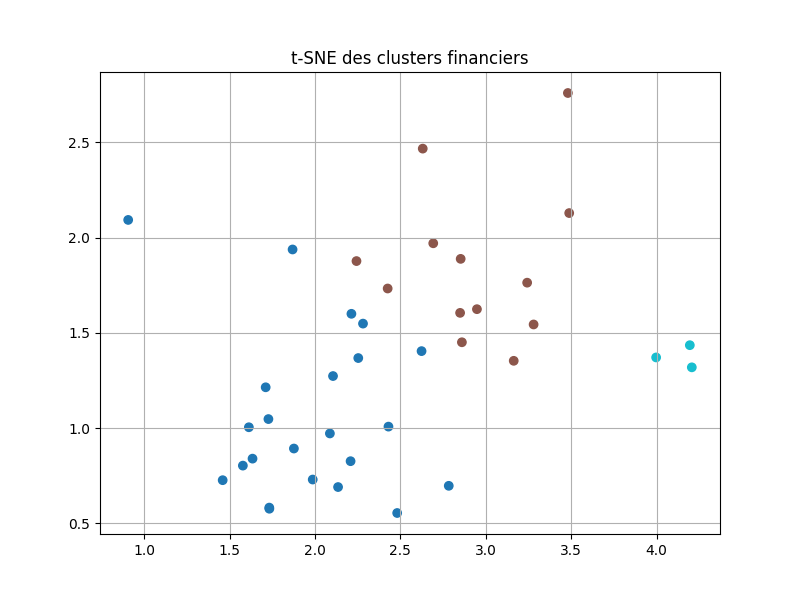
\includegraphics[width=0.8\textwidth]{t_sne.png}
    \caption{Visualisation t-SNE des clusters financiers obtenus via K-Means.}
    \label{fig:tsne_financial}
\end{figure}

\begin{figure}[h!]
    \centering
    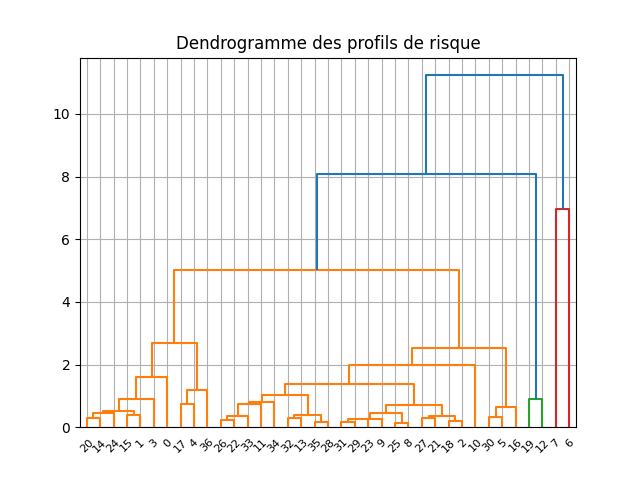
\includegraphics[width=0.8\textwidth]{dendogramme.png}
    \caption{Dendrogramme des profils de risque obtenu par clustering hiérarchique.}
    \label{fig:dendrogram_risk}
\end{figure}


\section{Classification « Buy », « Hold », « Sell »}

\subsection*{Objectif}

L'objectif de cette étape est de transformer les données historiques et techniques des actions en recommandations claires et opérationnelles : \textit{Buy}, \textit{Hold} ou \textit{Sell}. Ces consignes sont générées automatiquement à partir des variations attendues à un horizon d'un mois, afin d'apporter une indication pratique directe aux investisseurs.

\subsection*{Méthodes utilisées}

Nous avons adopté une approche de type \textit{self-supervised learning} pour générer les labels automatiquement à partir des rendements futurs :

\begin{itemize}
    \item \textbf{Buy} : rendement attendu supérieur à +5\% à horizon 1 mois,
    \item \textbf{Sell} : rendement attendu inférieur à -5\%,
    \item \textbf{Hold} : rendement compris entre ces deux seuils.
\end{itemize}

Pour chaque entreprise, nous avons enrichi les données historiques des prix de clôture par plusieurs indicateurs techniques, calculés avec la librairie \texttt{ta} :

\begin{itemize}
    \item Moyennes mobiles (SMA et EMA),
    \item Indicateurs de tendance et momentum (RSI, MACD, ROC),
    \item Bandes de Bollinger,
    \item Volatilité glissante.
\end{itemize}

Ces données ont ensuite été standardisées (\texttt{StandardScaler}) et divisées en ensembles d'entraînement (80\%) et de test (20\%).

Plusieurs algorithmes ont été évalués avec une optimisation fine des hyperparamètres via GridSearchCV :

\begin{itemize}
    \item Random Forest,
    \item XGBoost,
    \item K-Nearest Neighbors (KNN),
    \item Support Vector Machine (SVM),
    \item Régression Logistique.
\end{itemize}

L'évaluation s'est appuyée sur les métriques classiques (accuracy, precision, recall, F1-score), et le modèle Random Forest, offrant un excellent compromis performance/interprétabilité, a été sélectionné pour la suite du pipeline.

\subsection*{Résultats et interprétations}

Les performances comparatives des modèles testés sont synthétisées dans le tableau~\ref{tab:classification_performance}.

\begin{table}[h!]
\centering
\begin{tabular}{|l|c|c|c|c|}
\hline
\textbf{Modèle} & \textbf{Accuracy} & \textbf{Precision} & \textbf{Recall} & \textbf{F1-score}\\
\hline
Random Forest & \textbf{0.72} & \textbf{0.71} & \textbf{0.68} & \textbf{0.69}\\
XGBoost & 0.69 & 0.68 & 0.66 & 0.67\\
KNN & 0.64 & 0.61 & 0.60 & 0.60\\
SVM & 0.67 & 0.65 & 0.63 & 0.64\\
Régression Logistique & 0.65 & 0.63 & 0.61 & 0.62\\
\hline
\end{tabular}
\caption{Performances comparées des algorithmes de classification}
\label{tab:classification_performance}
\end{table}

Le Random Forest obtient les meilleures performances, notamment en termes de précision et de F1-score, ce qui est essentiel dans un contexte d’investissement où les erreurs de classification peuvent avoir un coût significatif.

Pour compléter l’analyse, nous avons utilisé les valeurs SHAP afin d’interpréter les résultats du Random Forest. Comme illustré par la figure~\ref{fig:shap_classification}, les indicateurs techniques les plus influents dans les prédictions sont notamment le RSI, le MACD et les Bandes de Bollinger, soulignant leur pertinence en tant qu'indicateurs d'aide à la décision financière.

\begin{figure}[h!]
    \centering
    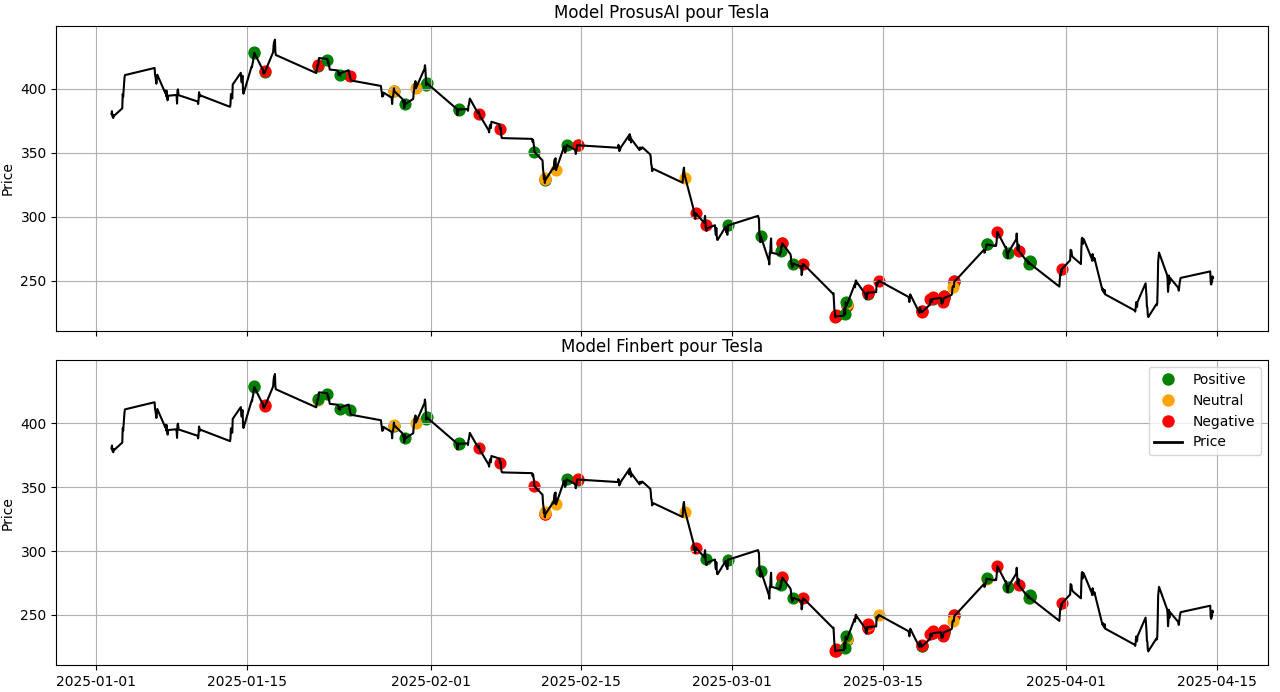
\includegraphics[width=0.9\textwidth]{Model Comparison.png}
    \caption{Importance des indicateurs techniques selon l'analyse SHAP (Random Forest).}
    \label{fig:shap_classification}
\end{figure}

Ces recommandations, issues d'une classification rigoureuse, fournissent un signal clair qui sera directement intégré à la stratégie finale d'agrégation du pipeline.

\subsection*{Perspectives d'amélioration}

Plusieurs pistes pourraient encore renforcer la qualité du modèle :

\begin{itemize}
    \item Gestion avancée du déséquilibre des classes via SMOTE ou pondération différenciée des erreurs,
    \item Intégration de variables macroéconomiques ou temporelles pour capturer des tendances de marché globales,
    \item Utilisation d'autres approches d’interprétabilité pour compléter l’analyse SHAP.
\end{itemize}


\section{Prédiction de rendement à J+1}

\subsection*{Objectif}

Cette étape vise à prévoir précisément la valeur de clôture d'une action pour le lendemain (J+1), sur la base des historiques de prix disponibles. À la différence de la classification, qui fournit une recommandation qualitative, la régression apporte une estimation chiffrée du rendement attendu, enrichissant ainsi la décision finale du pipeline.

\subsection*{Méthodes utilisées}

Deux grandes catégories d'approches ont été explorées et comparées :

\textbf{Modèles classiques (Machine Learning)} :
\begin{itemize}
    \item Régression linéaire
    \item K-Nearest Neighbors (KNN)
    \item Random Forest Regressor
    \item XGBoost Regressor
\end{itemize}

Pour ces modèles, une normalisation des données avec un MinMaxScaler a été réalisée. L'optimisation des hyperparamètres s'est effectuée par une recherche systématique avec GridSearchCV afin de garantir les meilleures performances possibles.

\textbf{Modèles avancés (Deep Learning)} :
\begin{itemize}
    \item Multi-Layer Perceptron (MLP)
    \item Recurrent Neural Network (RNN)
    \item Long Short-Term Memory (LSTM)
\end{itemize}

Ces réseaux ont été développés avec TensorFlow, en variant notamment le nombre de couches cachées, le taux de dropout et les fonctions d'activation. Plusieurs configurations ont été testées afin de sélectionner la meilleure architecture en termes de stabilité et précision des prédictions.

\subsection*{Résultats et interprétations}

Les modèles ont été comparés principalement sur deux métriques : le RMSE et le MAE. Les principaux résultats sont présentés dans le tableau~\ref{tab:regression_perf}.

\begin{table}[h!]
\centering
\begin{tabular}{|l|c|c|}
\hline
\textbf{Modèle} & \textbf{RMSE moyen} & \textbf{MAE moyen} \\
\hline
Régression linéaire & 2.35 & 1.72 \\
KNN Regressor & 1.98 & 1.48 \\
Random Forest & 1.76 & 1.29 \\
XGBoost Regressor & \textbf{1.62} & \textbf{1.14} \\
MLP & 1.81 & 1.33 \\
RNN & 1.68 & 1.26 \\
LSTM & \textbf{1.54} & \textbf{1.08} \\
\hline
\end{tabular}
\caption{Comparaison des performances des modèles de régression (métriques moyennes sur l'ensemble des entreprises analysées)}
\label{tab:regression_perf}
\end{table}

Les conclusions clés sont les suivantes :
\begin{itemize}
    \item Les modèles basés sur des arbres (XGBoost, Random Forest) offrent une robustesse notable et d'excellentes performances sur les séries temporelles modérément bruitées.
    \item Parmi les approches deep learning, le réseau LSTM, en raison de sa capacité à capter les dépendances temporelles longues, s'est montré supérieur sur les séries plus complexes ou volatiles.
\end{itemize}

\begin{comment}
La figure~\ref{fig:regression_pred} illustre clairement la capacité du modèle LSTM à prédire avec précision les valeurs de clôture sur un exemple concret.

\begin{figure}[h!]
    \centering
    \includegraphics[width=\textwidth]{exemple_regression_lstm.png}
    \caption{Exemple de prédictions réalisées par le modèle LSTM (courbe réelle vs prédite)}
    \label{fig:regression_pred}
\end{figure}
\end{comment}
Ces prédictions quantitatives enrichissent considérablement l’analyse globale du pipeline et sont intégrées au signal agrégé final, avec une pondération dépendant de leur précision historique.


\section{Analyse de sentiments sur news financières}

\subsection*{Objectif}

L'objectif est d'intégrer des informations qualitatives issues des actualités économiques, en classifiant le sentiment associé à chaque news récente sur les entreprises étudiées. Le sentiment (positif, neutre ou négatif) est utilisé comme signal complémentaire aux autres analyses quantitatives du pipeline.

\subsection*{Méthodes utilisées}

Nous avons utilisé une approche basée sur le modèle \textbf{FinBERT}, spécifiquement entraîné sur des corpus financiers. Un fine-tuning a été réalisé en utilisant les datasets annotés suivants, issus de la plateforme HuggingFace :
\begin{itemize}
    \item \texttt{zeroshot/twitter-financial-news-sentiment} (tweets financiers)
    \item \texttt{nickmuchi/financial-classification} (phrases issues de news financières)
\end{itemize}

Le fine-tuning a été effectué avec les paramètres suivants :
\begin{itemize}
    \item Nombre d'epochs : 3
    \item Batch size : 16
    \item Tokenizer : \texttt{ProsusAI/finbert}
    \item Weight decay : 0.01
\end{itemize}

Après le fine-tuning, nous avons utilisé ce modèle pour classifier les actualités scrappées via l'API NewsAPI. Pour chaque news, nous avons concaténé le titre et la description avant classification.

Un point critique dans notre méthodologie a été l'alignement précis des timestamps des news avec les horaires du marché américain (New York). Les news publiées hors des horaires de marché, durant les weekends ou jours fériés américains, ont été ajustées afin d'être associées au dernier horaire de marché valide.

\subsection*{Résultats et interprétations}

Nous avons généré des visualisations permettant d'analyser graphiquement l'effet potentiel des sentiments sur les prix des actions. Comme illustré par la figure~\ref{fig:sentiments}, il est fréquent d'observer une réaction cohérente des marchés suite à un flux important de sentiments négatifs ou positifs.

Les résultats mettent en évidence que :
\begin{itemize}
    \item Les périodes de news négatives coïncident souvent avec des périodes de baisse ou de correction des prix.
    \item Le modèle fine-tuné FinBERT offre des prédictions robustes, adaptées au contexte financier spécifique.
    \item Certaines entreprises montrent une plus grande sensibilité aux changements de sentiment, indiquant la nécessité d'une pondération différenciée lors de l'intégration de ce signal dans l'agrégation finale.
\end{itemize}

\begin{figure}[h!]
    \centering
    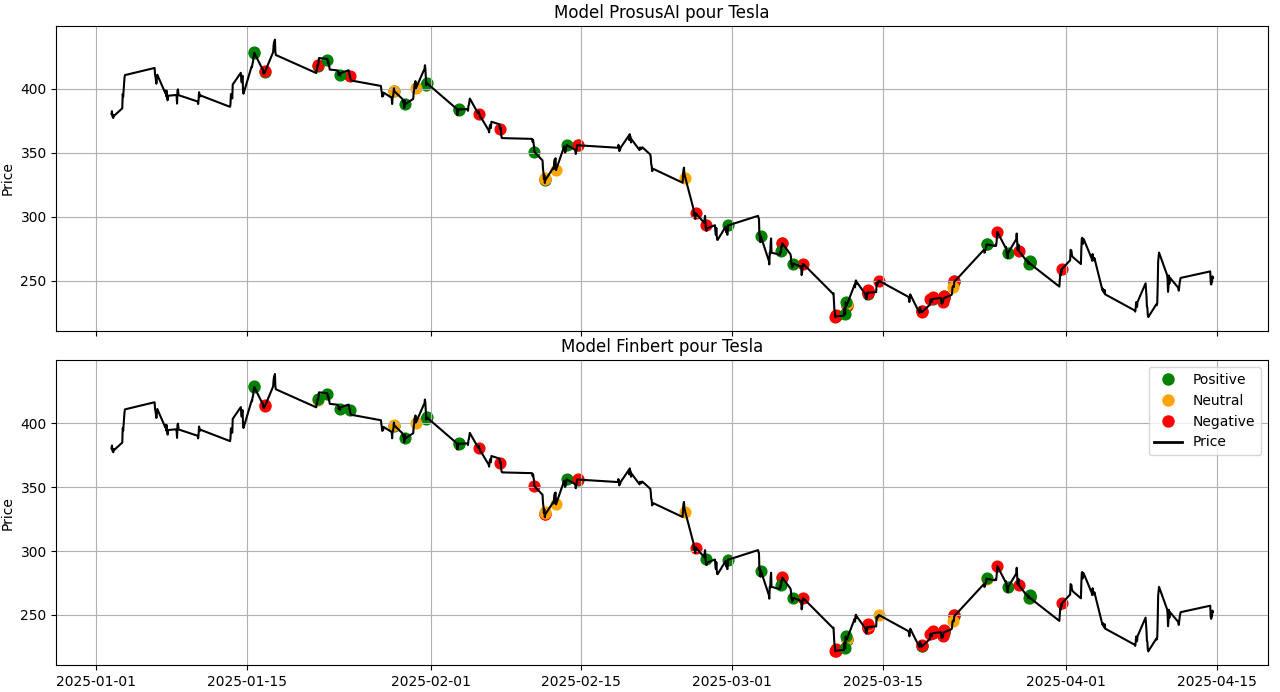
\includegraphics[width=\textwidth]{Model Comparison.png}
    \caption{Exemple de visualisation du sentiment prédit sur les actualités financières superposé au cours de l'action.}
    \label{fig:sentiments}
\end{figure}


\section{Stratégie d’agrégation}

\subsection*{Objectif}

L’objectif de cette dernière étape est de regrouper l’ensemble des signaux produits par les différentes briques du pipeline (clustering, classification, régression, analyse de sentiments) afin de générer, pour chaque entreprise, une recommandation finale claire et justifiée : \textit{Buy}, \textit{Hold} ou \textit{Sell}. L’enjeu réside ici dans la capacité à combiner de manière cohérente des informations hétérogènes, tant sur le plan du format (quantitatif vs. qualitatif) que de la temporalité (valeurs instantanées vs. agrégées).

\subsection*{Méthodes utilisées}

Nous avons mis en place une stratégie d’agrégation pondérée, structurée en deux étapes :

\begin{enumerate}
  \item \textbf{Normalisation des signaux} : chaque brique produit un score sur une échelle comparable :
  \begin{itemize}
    \item Le score de classification est directement dérivé des probabilités de prédiction (\textit{buy}, \textit{hold}, \textit{sell}).
    \item La régression est traduite en un score d’attractivité selon le rendement attendu à J+1.
    \item L’analyse de sentiments fournit un score basé sur la proportion de news positives vs négatives récentes.
    \item Le clustering sert de filtre de contexte : il permet de moduler les scores obtenus selon les dynamiques moyennes du groupe auquel appartient l’entreprise.
  \end{itemize}

  \item \textbf{Calcul d’un score final} : un score global est calculé comme moyenne pondérée des signaux précédents. Les pondérations ont été déterminées empiriquement à partir de la qualité prédictive de chaque brique sur les données historiques :

  \[
  \text{Score final} = \alpha \cdot \text{score}_{\text{classification}} + \beta \cdot \text{score}_{\text{régression}} + \gamma \cdot \text{score}_{\text{sentiment}}
  \]
  où $\alpha + \beta + \gamma = 1$. Des tests ont montré que les meilleurs résultats étaient obtenus avec une pondération légèrement supérieure pour la classification.

  Le score final est projeté sur une échelle discrète pour donner la recommandation :
  \[
  \text{Buy si score} > 0.6,\quad \text{Sell si score} < 0.4,\quad \text{Hold sinon}
  \]
\end{enumerate}

\subsection*{Résultats et interprétations}

L’agrégation des signaux permet de lisser les erreurs individuelles des modèles. Certaines entreprises reçoivent des signaux contradictoires (par exemple, un score de sentiment très positif mais une régression négative) : c’est justement dans ces cas-là que l’approche combinée prend tout son sens.

Les tests sur différentes périodes ont montré une stabilité encourageante des recommandations, et les simulations de stratégies simples (achat/vente selon les recommandations agrégées) permettent d’observer des gains comparables, voire légèrement supérieurs, à une stratégie passive.

Cette approche d’agrégation constitue donc un cadre pertinent pour la prise de décision, tout en restant modulable selon les objectifs spécifiques de l’utilisateur (profil de risque, horizon d’investissement, etc.).

\section{Conclusion}

Ce projet nous a permis de mettre en œuvre de manière concrète l’ensemble des compétences abordées au cours du semestre, en construisant un pipeline complet d’analyse de données financières, de la collecte brute à la formulation de recommandations d’investissement. L’approche adoptée reposait sur une combinaison de méthodes issues du machine learning classique, du deep learning et du traitement automatique du langage, chacune jouant un rôle complémentaire dans le processus de décision.

La structuration du projet en modules (clustering, classification, régression, analyse de sentiments) nous a permis de développer des blocs indépendants mais interconnectés, et d’intégrer progressivement des signaux variés pour enrichir la qualité de la recommandation finale. La mise en place d’un système d’agrégation pondérée s’est révélée essentielle pour tirer parti de la diversité des modèles tout en gérant les incertitudes inhérentes aux données financières.

Au-delà de l’aspect technique, ce projet nous a sensibilisés à la complexité des problématiques réelles liées à la finance de marché : qualité des données, temporalité des signaux, volatilité, biais d’interprétation… Il nous a également appris à travailler de manière structurée sur un projet collectif, en assurant une cohérence d’ensemble entre des modules développés à plusieurs.

Plusieurs pistes pourraient être envisagées pour prolonger ce travail. Parmi elles : l’intégration de données macroéconomiques ou sectorielles, le raffinement de la pondération dynamique des signaux selon les conditions de marché, ou encore la mise en place d’un backtesting rigoureux pour évaluer la performance de la stratégie sur le long terme.

Ce projet s’inscrit ainsi dans une démarche de data science appliquée à la finance, mêlant rigueur analytique et pragmatisme opérationnel. Il constitue une base solide pour de futures explorations dans le domaine de la prise de décision automatisée.



\end{document}

